% do not change these two lines (this is a hard requirement
% there is one exception: you might replace oneside by twoside in case you deliver 
% the printed version in the accordant format
\documentclass[11pt,titlepage,oneside,openany]{book}
\usepackage{times}


\usepackage{graphicx}
\usepackage{latexsym}
\usepackage{amsmath}
\usepackage{amssymb}

\usepackage{ntheorem}

% \usepackage{paralist}
\usepackage{tabularx}
\usepackage{url}

% this packaes are useful for nice algorithms
\usepackage{algorithm}
\usepackage{algorithmic}

% well, when your work is concerned with definitions, proposition and so on, we suggest this
% feel free to add Corrolary, Theorem or whatever you need
\newtheorem{definition}{Definition}
\newtheorem{proposition}{Proposition}


% its always useful to have some shortcuts (some are specific for algorithms
% if you do not like your formating you can change it here (instead of scanning through the whole text)
\renewcommand{\algorithmiccomment}[1]{\ensuremath{\rhd} \textit{#1}}
\def\MYCALL#1#2{{\small\textsc{#1}}(\textup{#2})}
\def\MYSET#1{\scshape{#1}}
\def\MYAND{\textbf{ and }}
\def\MYOR{\textbf{ or }}
\def\MYNOT{\textbf{ not }}
\def\MYTHROW{\textbf{ throw }}
\def\MYBREAK{\textbf{break }}
\def\MYEXCEPT#1{\scshape{#1}}
\def\MYTO{\textbf{ to }}
\def\MYNIL{\textsc{Nil}}
\def\MYUNKNOWN{ unknown }
% simple stuff (not all of this is used in this examples thesis
\def\INT{{\mathcal I}} % interpretation
\def\ONT{{\mathcal O}} % ontology
\def\SEM{{\mathcal S}} % alignment semantic
\def\ALI{{\mathcal A}} % alignment
\def\USE{{\mathcal U}} % set of unsatisfiable entities
\def\CON{{\mathcal C}} % conflict set
\def\DIA{\Delta} % diagnosis
% mups and mips
\def\MUP{{\mathcal M}} % ontology
\def\MIP{{\mathcal M}} % ontology
% distributed and local entities
\newcommand{\cc}[2]{\mathit{#1}\hspace{-1pt} \# \hspace{-1pt} \mathit{#2}}
\newcommand{\cx}[1]{\mathit{#1}}
% complex stuff
\def\MER#1#2#3#4{#1 \cup_{#3}^{#2} #4} % merged ontology
\def\MUPALL#1#2#3#4#5{\textit{MUPS}_{#1}\left(#2, #3, #4, #5\right)} % the set of all mups for some concept
\def\MIPALL#1#2{\textit{MIPS}_{#1}\left(#2\right)} % the set of all mips





\begin{document}

\pagenumbering{roman}
% lets go for the title page, something like this should be okay
\begin{titlepage}
	\vspace*{2cm}
  \begin{center}
   {\Huge Locating Companies \\}
	\vspace*{0.5cm}
   {\large  interlinking ProductDB with DBPedia based on product categories \\}
   \vspace{2cm} 
   \vspace{2cm}
   {written by\\
    Markus Dietsche 1513384 \\
    Dandan Li 1486051\\
   }
   \vspace{1cm} 
   {submitted to the\\
    Data and Web Science Group \\
    Prof.\ Dr.\ Paulheim\\
    University of Mannheim\\} \vspace{2cm}
   {December 2015}
  \end{center}
\end{titlepage} 

% no lets make some add some table of contents
\tableofcontents
\newpage

\listofalgorithms

\listoffigures

\listoftables

% evntuelly you might add something like this
% \listtheorems{definition}
% \listtheorems{proposition}

\newpage


% okay, start new numbering ... here is where it really starts
\pagenumbering{arabic}

\chapter{Application domain and goals}
\label{cha:goal}

Most of the text in this example of a master thesis is quote from 'The Extremes of Good and Evil' (Cicero). Besides this text you find some usage examples in the following sections.

\begin{itemize}
	\item A table can be found in Section \ref{sec:query}. This example (Table \ref{tab:confonly}) is only a suggestion. You are allowed to format your tables in your preferred style.
	\item An example of an algorithm is depicted in Section \ref{sec:challenge}. Again, you are allowed to use a different style for algorithms, but the style we used to display Algorithm \ref{cha:dataset} looks quite nice.
	\item Chapter \ref{cha:example} demontrates how to refer to chapters and algorithms and other elements of your thesis.
	\item You should always place definitions, propositions, and whatever might be useful in an appropriate environment.  Examples can be found in section \ref{sec:idea}.
\end{itemize}




 
\section{Targeted Users}
 
it's  a footnote and url
\footnote{http://productDB.org/}


Tutorials\footnote{\url{http://latex.hpfsc.de}}.  
 here is sth.wrong with url on my pc


\section{Problems Description}

 

\section{Demand Analysis}



\chapter{Datasets used}
\label{cha:dataset}




\section{Datasets description}
\label{sec:datadesc}

 dicussion requires a precise definition.
\begin{definition}
\label{def:good}
An entity is good if it is not an evil entity.
\end{definition}
In a similar way an evil entity can be defined in the following way.



\section{Dataset Access Methods}
\label{sec:dataaccess}


\section{Dataset Combination}
\label{sec:datacomb}


\begin{figure}
	\begin{center}
	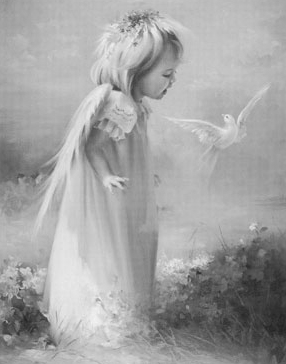
\includegraphics[width=5cm]{good.png}
	\caption[Angel]{Child Angel and a white dove.}
	\label{fig:angel}
	\end{center}
\end{figure}



\chapter{Techniques Used}
\label{cha:technique}



\section{Reasoning}
\label{sec:reasoning}


\section{Search}
\label{sec:search}

\section{External Services}
\label{sec:service}

\textit{Remark: A more elaborated software could use e.g. OpenStreetMap to inquiry the exact address based on the DBPedia results.}



\chapter{Example results}
\label{cha:example}


\paragraph{Example} 
an inquery for “soft-drinks” will have a result set containing:
\begin{verbatim}
dbo:locationCity : 
(dbr:Atlanta, 
dbr:Georgia_(U.S._state), 
dbr:Coca-Cola_headquarters)
\end{verbatim}


\section{Outcome}
\label{sec:outcome}



\section{User Queries}
\label{sec:query}



\begin{table}[h]

\begin{center}
\begin{tabular*}{\textwidth}{@{\extracolsep{\fill}}>{\scriptsize}l|>{\scriptsize}c>{\scriptsize}c>{\scriptsize}c|>{\scriptsize}c>{\scriptsize}c>{\scriptsize}c>{\scriptsize}c} 
& \multicolumn{3}{>{\scriptsize}c|}{Baselines} & \multicolumn{4}{>{\scriptsize}c}{Decision Tree} \\\hline
Ontology & M(edian) & G(ood) & E(vil) & results & $\Delta$-M & $\Delta$-G & $\Delta$-E \\\hline\hline
\#301 & 0.825 & 0.877 & 0.877 & 0.855 & +0.030 & -0.022 & -0.022 \\\hline
\#302 & 0.709 & 0.753 & 0.753 & 0.753 & +0.044 & +0.000 & +0.000 \\\hline
\#303 & 0.804 & 0.860 & 0.891 & 0.816 & +0.012 & -0.044 & -0.075 \\\hline
\#304 & 0.940 & 0.961 & 0.961 & 0.967 & +0.027 & +0.006 & +0.006 \\\hline
\bfseries Average & \bfseries 0.820 & \bfseries 0.863 & \bfseries 0.871 & \bfseries 0.848 & \bfseries +0.028 & \bfseries -0.015 & \bfseries -0.023 

\end{tabular*}
\caption[Good vs. Evil]{Comparison between the Good and the Evil}
\label{tab:confonly}
\end{center}
\end{table}



\chapter{known limitations}
\label{cha:limits}





\section{limited domains}
\label{sec:lidomain}



\section{queries can't be answered}
\label{sec:unquery}

\section{Reason}
\label{sec:reason}


\section{Possible Solutions}
\label{sec:solution}



\chapter{Lessons learned}
\label{cha:lessons}

\section{Challenges}
\label{sec:challenge}

\section{Biggest Obstacles}
\label{sec:obstacle}

\section{More ideas}
\label{sec:idea}

\bibliographystyle{plain}
\bibliography{thesis-ref}


\appendix

\chapter{Program Code / Resources}
\label{cha:appendix-a}

The source code, a documentation, some usage examples, and additional test results are available at ...

They as well as a PDF version of this thesis is also contained on the CD-ROM attached to this thesis.

\chapter{Further Experimental Results}
\label{cha:appendix-b}

In the following further experimental results are ...


\newpage

\end{document}
